\documentclass{jps-cp}
\usepackage{txfonts} %Please comment out this line unless the txfonts package is availabe in your LaTeX system.
\usepackage{url}
\usepackage{multirow}
\usepackage{array, booktabs}
\usepackage{wrapfig}
\usepackage{color}

\makeatletter
\newcommand{\figcaption}[1]{\def\@captype{figure}\caption{#1}}
\newcommand{\tblcaption}[1]{\def\@captype{table}\caption{#1}}

\title{New analysis method of TPC data using neural network}

\author{
  Takanobu \textsc{Doi}$^{1}$, Takahiro \textsc{Kawabata}$^{2}$, Tatsuya \textsc{Furuno}$^{3}$,
  Yuki \textsc{Fujikawa}$^{1}$, Kento \textsc{Inaba}$^{1}$, Motoki \textsc{Murata}$^{3}$,
  Shintaro \textsc{Okamoto}$^{1}$, and Akane \textsc{Sakaue}$^{1}$}

\inst{
  $^{1}$Department of Physics, Kyoto University, Kyoto, Kyoto 606-8502, Japan \\
  $^{2}$Department of Physics, Osaka University, Toyonaka, Osaka 540-0043, Japan \\
  $^{3}$Research Center for Nuclear Physics, Osaka University, Ibaraki, Osaka 567-0047, Japan }

\email{doi.takanobu.68x@st.kyoto-u.ac.jp}

\recdate{November 18, 2019} % Write received date here

\abst{
  The MAIKo time projection chamber (TPC) enables us to project three-dimensional
  tracks of charged particles onto two planes perpendicular
  and parallel to the beam axis, and to acquire these projections as two images.
  It is, therefore, necessary to analyze these two-dimensional images 
  to reconstruct the original three-dimensional tracks of the charged particles.
  These images are often analyzed with the Hough transformation.
  This method requires a complex algorithm and a large computing power.
  In the present work, we developed a new method to analyze track images obtained
  by the MAIKo TPC using neural networks which are widely employed for the image recognition.
  This new method successfully makes the analysis faster and more accurate than the previous method.
} % Write abstract here

\kword{neural networks, time projection chamber (TPC), active target, MAIKo TPC} % Write keywords here

\begin{document}
\maketitle

\section{Introduction}
\begin{wrapfigure}{r}{15zw}
  \vspace{0zw}
  \centering
  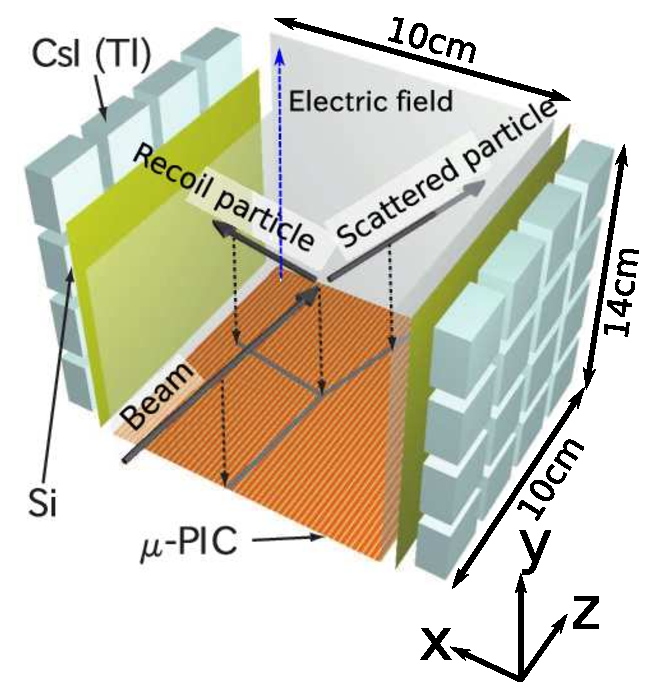
\includegraphics[clip, width=15zw]{eps/MAIKo_v2.eps}
  \caption{Schematic view of the MAIKo TPC.}
  \label{fig:MAIKo}
  \vspace{-2zw}
\end{wrapfigure}
Time projection chambers (TPCs) are widely used to detect tracks of charged particles.
We developed a TPC using a micro pixel chamber ($\mu$-PIC)~\cite{mupic} named
MAIKo ($\mu$-PIC based active target for inverse kinematics.)~\cite{MAIKo}
for experiments with unstable nuclei.
Figure \ref{fig:MAIKo} shows a schematic view of the MAIKo TPC.
When charged particles pass through the MAIKo TPC filled with the detection gas,
electrons and ions are generated along the particle tracks.
These electrons are drifted downward by an electric field and
gas-amplified on the surface of the $\mu$-PIC.
The anode and cathode electrodes of the $\mu$-PIC are segmented into 256 strips, respectively,
which are arranged orthogonally.
These strips are aligned at 400-$\rm{\mu m}$ intervals.
Anode strips are parallel to $x$-axis and 
cathode strips are parallel to $z$-axis as shown in Fig.~\ref{fig:MAIKo}. 
Electric signals induced by the multiplied electrons
and ions are read out through the anode and 
cathode strips to determine the $x$ and $z$ position of the particle tracks.
The vertical position of the tracks along the $y$-axis is determined 
from the drift time of the electrons.
Thus, the three-dimensional tracks are reconstructed from $x$-, $y$-, and $z$-coordinates.

Incident nuclei are scattered by target particles in the gas of the TPC as shown in Fig.~\ref{fig:MAIKo}, 
{\it i.e.} the gas plays a role of the target gas.
In forward scatterings where the momentum transfer is small,
scattered particles escape from the sensitive volume of the TPC, but low-energy recoil particles stop inside.
Since reaction points are inside the sensitive volume of the TPC,
it is possible to detect even low-energy particles over a large solid angle.
$\rm{H}_{2}$ or $\rm{He}$ gas is widely used as a target gas
but operation of TPC with pure $\rm{H}_{2}$ or $\rm{He}$ gas is prone to discharge.
Usually, quenching gas with a high tolerance for electric discharges
like $\rm{CO}_{2}$ or iso-butane is mixed with a target gas
for stable operation of the TPC although the quenching gas causes background events.
Recently, the elastic and inelastic alpha scattering on ${}^{10}\rm{C}$ at forward center-of-mass angles
were measured with the MAIKo TPC at Research Center for Nuclear Physics (RCNP), Osaka University.
In this experiment, $\rm{He}$ (96\%) was used as the target gas, and $\rm{CO}_{2}$ (4\%) was used as the quenching gas.

The tracks of charged particles in each event were projected onto the $z$-$y$ and $y$-$z$ planes 
that are perpendicular to the anode and cathode strips, and were recorded as the anode and cathode images.
Figures \ref{fig:true} and \ref{fig:false} are examples of the acquired images.
These black-and-white images with $1024\times 256$ pixels present the hit pattern of the 256 strips 
on the anode and cathode recorded
at every $10~\rm{ns}$ for the duration of $10~\rm{ns}\times 1024 = 10.24~\rm{\mu s}$.
Figure \ref{fig:true} shows a ${}^{10}\rm{C}+\alpha$ event
in which the incident ${}^{10}\rm{C}$ beam was scattered at the small angle from the beam axis and the $\alpha$ particle was
recoiled at the large angle.
On the other hand, Figure~\ref{fig:false} shows a background event due to a heavy nucleus in the quenching gas (C or O).
The incident ${}^{10}\rm{C}$ beam should be scattered from a heavy nucleus because the scattering angle was large.
If the incident ${}^{10}\rm{C}$ had been scattered with ${}^{4}\rm{He}$,
it would not have been scattered at such a large angle.

For the ${}^{10}\rm{C}+\alpha$ events, the energy and emission angle of the recoil $\alpha$ particle must
be determined to obtain the spectroscopic information such as the excitation energy of ${}^{10}\rm{C}$
and the scattering angle in the center-of-mass system.
The energy of the recoil $\alpha$ particle is determined from the length of the track 
in the detection gas consisting of the target gas and the quenching gas,
while the emission angle is determined from the opening angle between the incident particle 
and the recoil $\alpha$ particle.
The anode and cathode images were analyzed with the following two steps;
selecting true ${}^{10}\rm{C}+\alpha$ events,
and determining the length and the emission angle of $\alpha$ particle from
the anode and cathode images.
However, the method using the Hough transformation required a lot of efforts to
do these two analyses.
Therefore, we have developed a new method using neural networks which are widely employed for the image recognition.
The neural networks were also employed for the analysis of TPC data in recent years~\cite{attpc}.

\begin{figure}
  \centering
  \begin{minipage}{0.45\columnwidth}
    \centering
    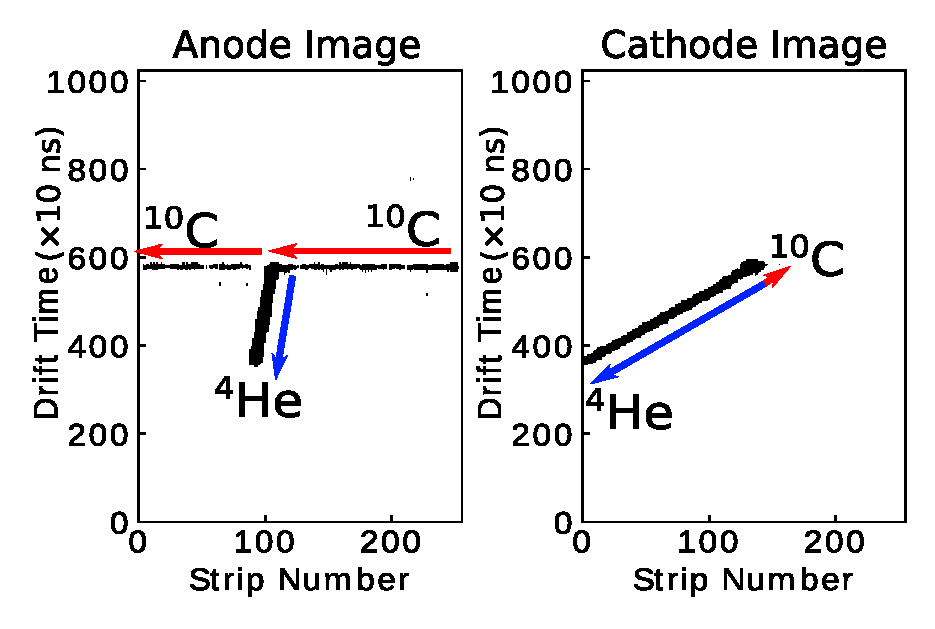
\includegraphics[clip, width=0.9\columnwidth]{eps/true.eps}
    \caption{Typical anode and cathode images recorded in a ${}^{10}\rm{C}+\alpha$ event.}
    \label{fig:true}
  \end{minipage}
  \hfill
  \begin{minipage}{0.45\columnwidth}
    \centering
    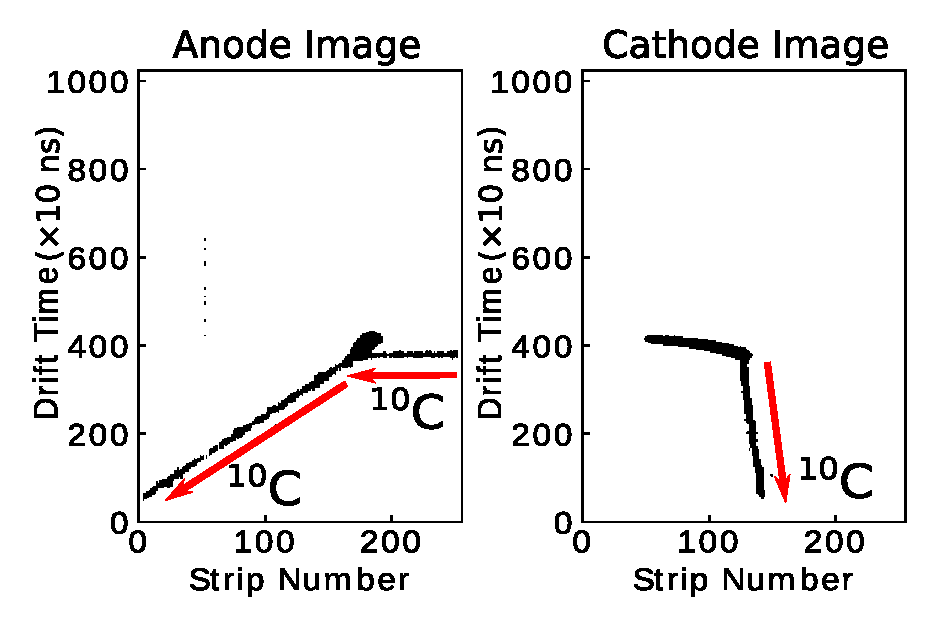
\includegraphics[clip, width=0.9\columnwidth]{eps/false.eps}
    \caption{Same as Fig.~\ref{fig:true} but recorded in a background event.}
    \label{fig:false}
  \end{minipage}
\end{figure}

\section{Previous method using the Hough transformation}
Previously, the Hough transformation had been employed in order to
select the ${}^{10}\rm{C}+\alpha$ events and to determine tracks.
The Hough transformation is one of methods to find lines in an image.
A hit pixel at $(x_{i}, y_{i})$ in the image
is transformed into
a curved line in the $(\theta, r)$ parameter space (Hough space)
according to Eq. (\ref{eq:real2hough}).
\begin{equation}
  \label{eq:real2hough}
  r = x_{i}\cos\theta+y_{i}\sin\theta. 
\end{equation}
A point at $(\theta_{j}, r_{j})$ in the Hough space corresponds to a straight line
in the original image as given by Eq. (\ref{eq:hough2real}).
\begin{equation}
  \label{eq:hough2real}
  y = -\frac{x}{\tan\theta_{j}}+\frac{r_{j}}{\sin\theta_{j}}. 
\end{equation}
When the pixels in the anode or cathode image lie on a straight line,
their transformed curves intersect at one point at $(\theta_{j}, r_{j})$ in the Hough space.
Thus, the intersecting point in the Hough space gives the particle track according to Eq. (\ref{eq:hough2real}).

It is possible to select the ${}^{10}\rm{C}+\alpha$ events by
utilizing information about the straight lines extracted from the anode and cathode images such as
the number, position, angle and length.
Once the ${}^{10}\rm{C}+\alpha$ events are selected, the energy and angle of the recoil $\alpha$ particle
are determined from the images to calculate the excitation energy and the scattering angle in the center-of-mass system.
However, the previous method with the Hough transformation requires a complicated algorithm with many adjustable parameters,
and the optimization of these parameters needs a large computing power.
It takes about 24 hours to optimize the parameters using 100 CPUs
in the computing system at RCNP, 
and about one second to process the anode and cathode images from one event using one CPU after the parameter optimization.
The accuracy of the event selection was rated 89\% using 3,000 events,
which were tagged with human eyes.

\section{New method using neural networks}
The previous method has problems of requiring a complex algorithm and a large computing power.
We developed a new method using neural networks.
Using neural networks, it might be possible to recognize images
considering many features of tracks without any complicated algorithms.
Once a neural network trained, the neural network is expected to recognize images faster and more accurate than the previous method.


\vspace{0zw}
\begin{figure}
  \centering
  \begin{minipage}{0.4\columnwidth}
    \centering
    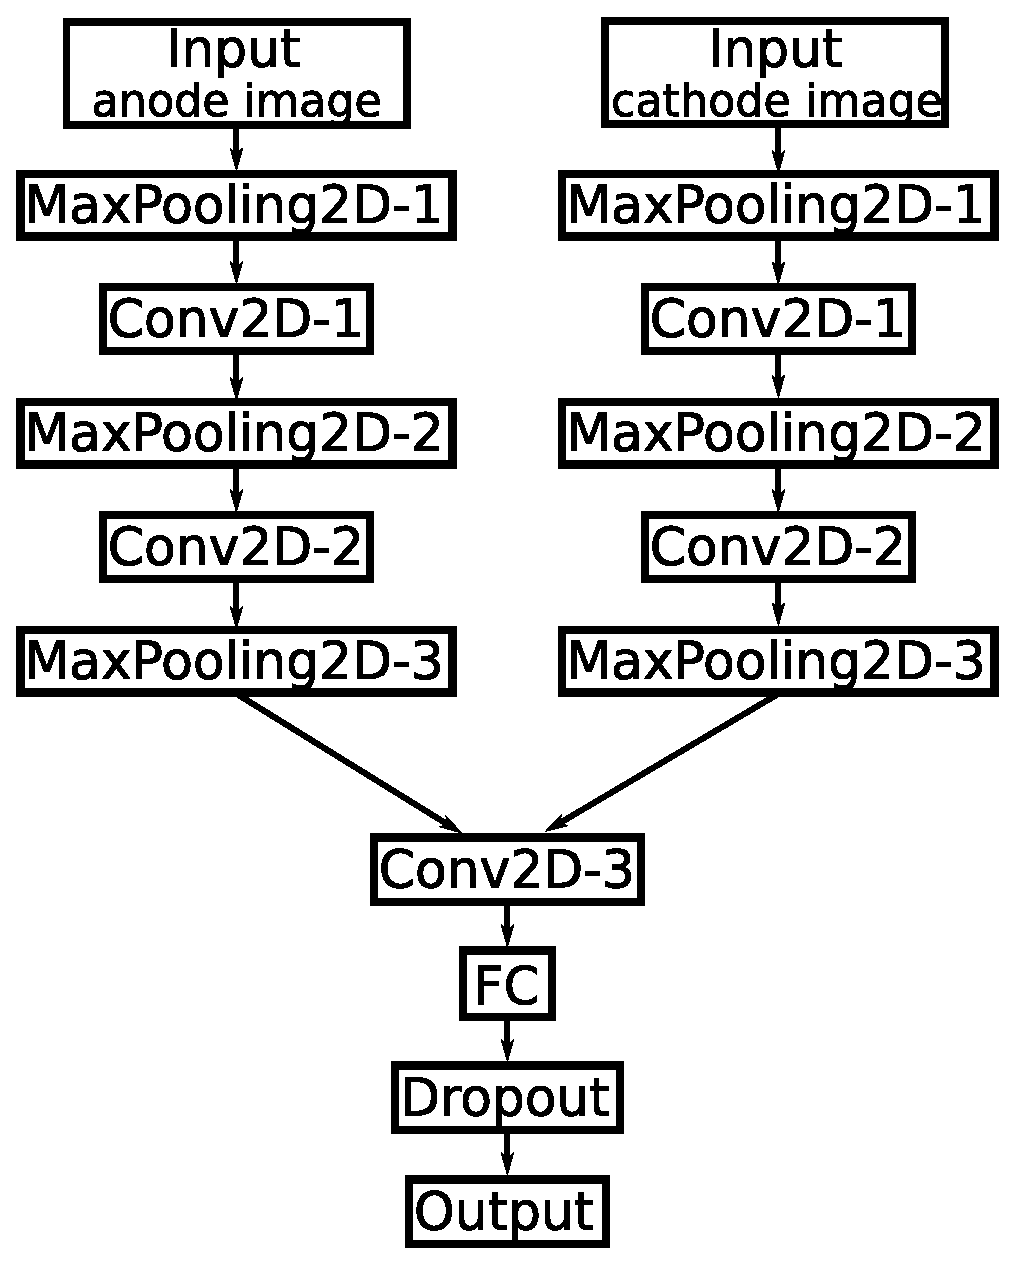
\includegraphics[clip, width=0.9\columnwidth]{eps/event_selection_v2.eps}
    \caption{Schematic structure of the neural network for the event selection.
      The details are explained in the text.}
    \label{fig:selection}
  \end{minipage}
  \hfill
  \begin{minipage}{0.4\columnwidth}
    \centering
    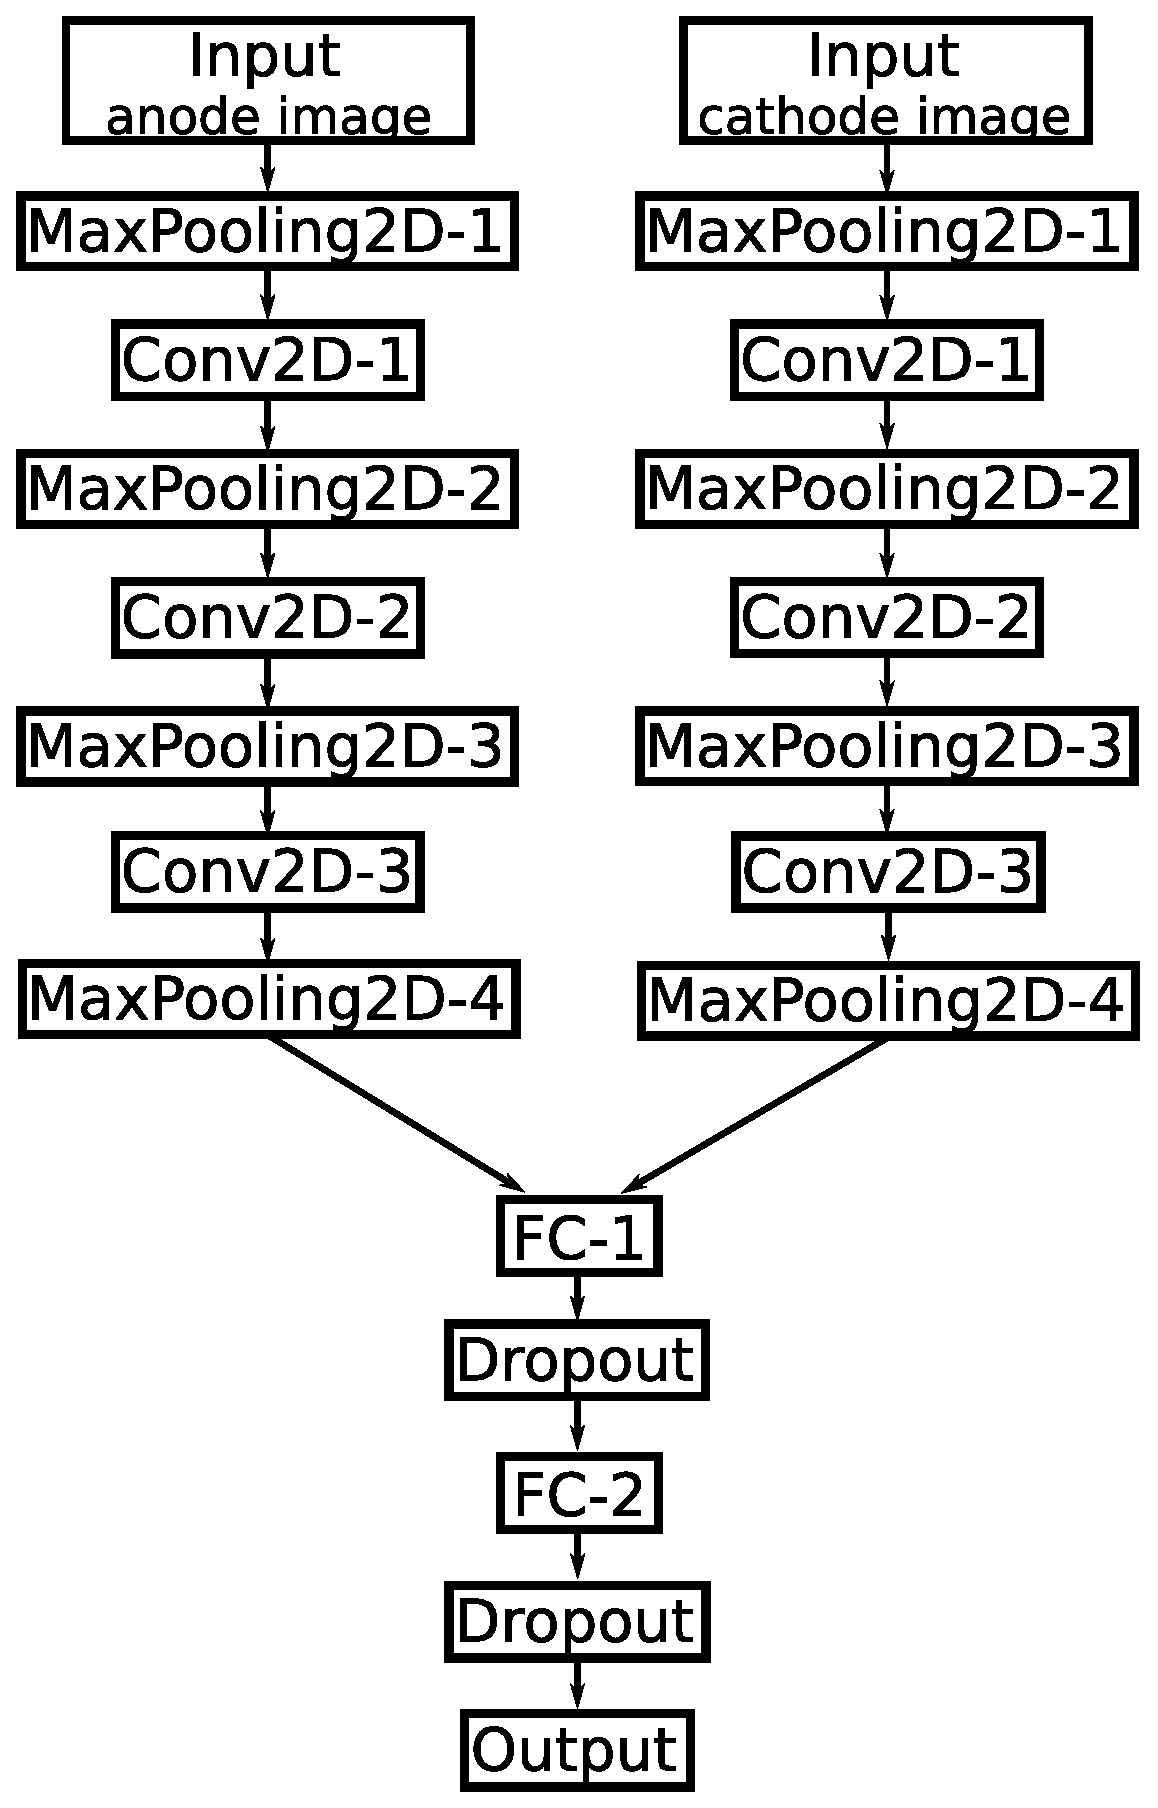
\includegraphics[clip, width=0.9\columnwidth]{eps/point_detection_v2.eps}
    \caption{Schematic structure of the neural network for the track determination.
      The details are explained in the text.}
    \label{fig:extraction}
  \end{minipage}
\end{figure}

We used convolutional neural networks (CNNs) that are useful for image recognition~\cite{lenet,alexnet}.
Since the analysis consists of the event selection and the track determination,
we used two networks.
Figures \ref{fig:selection} and \ref{fig:extraction} show
the networks for the event selection and the track determination, respectively.
Neural networks generally consist of the input layer, the output layer, and the hidden layers.
Because the anode and cathode images have different features,
the networks have two branches.
We inputted a pair of images from the MAIKo TPC to the neural networks.
The network for the event selection has 16 layers and the network for the track determination has 21 layers.
``MaxPooling2D'', ``Conv2D'', ``FC'', and ``Dropout'' in Figs.~\ref{fig:selection} and \ref{fig:extraction}
mean the maxpooling layer, convolutional layer, fully connected layer, and dropout layer respectively.
The maxpooling layers reduce the size of feature maps by taking the maximum value.
The convolutional layers emphasize the features of the input maps through filters.
The fully connected layers process the features from the previous layer and pass them to the next layer.
The dropout layers block some of the signal from the previous layer to the next layer to avoid overfitting.
See Ref.~\cite{conv,dropout} for details about the function of each layer.
The structures of the networks in Figs. \ref{fig:selection} and \ref{fig:extraction}, {\it i.e.}
the number and the types of the layers were
optimized to achieve the highest accuracy in the analysis.

In the event selection, the neural network determined a probability that the pair of images were taken
in the ${}^{10}\rm{C}+\alpha$ event.
If the probability was larger than 50\%, the event was regarded as the ${}^{10}\rm{C}+\alpha$ scattering.
This network was trained and evaluated with the images from 3,000 events of the ${}^{10}{\rm C}+\alpha$
events and background events tagged by human eyes,
which were the same images as those used in the previous method.
The 2,700 events were used for the training, and the other 300 events were for the evaluation.
In the track determination, the network outputted the coordinates of two endpoints of
a track of a recoil $\alpha$ particle in a ${}^{10}\rm{C}+\alpha$ event.
This network was trained and evaluated with the images from 4,566 events of the ${}^{10}\rm{C}+\alpha$ events.
The coordinates of the track end points in these events had been determined by the previous method
before the new analysis with the neural network.
The 3,012 events were used for the training, and the other 1,554 events were for the evaluation.
We used Intel Core i7, Nvidia GeForce GTX 1080Ti, Ubuntu 18.04 LTS, and
TensorFlow~\cite{tensorflow} + Keras~\cite{keras} in the present analysis.

\section{Result}
\begin{wrapfigure}{r}{25zw}
  \vspace{-3zw}
  \centering
  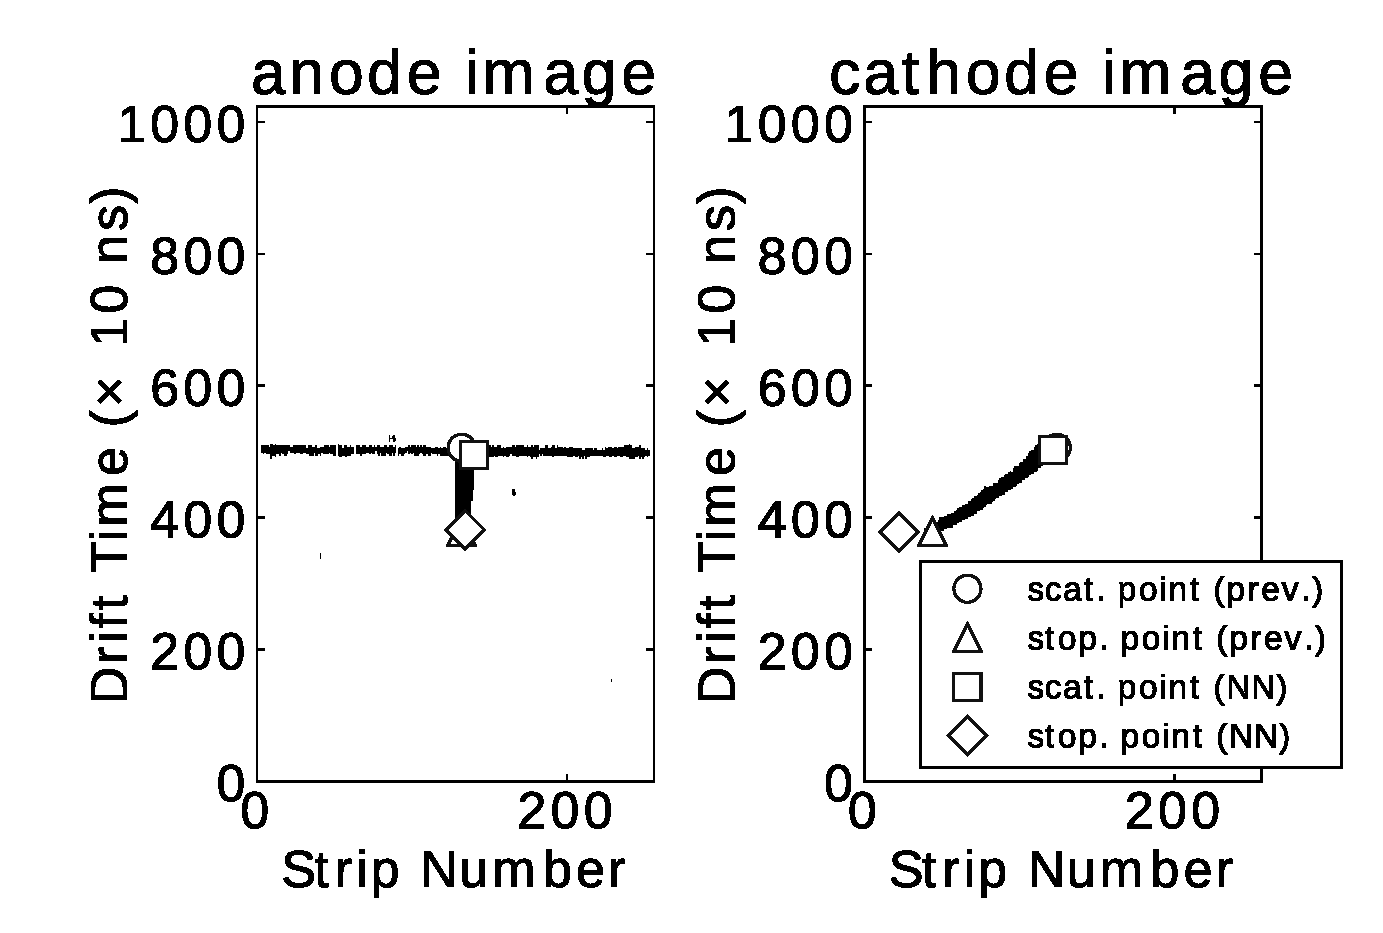
\includegraphics[clip, width=25zw]{eps/compare_mono_v4.eps}
  \caption{Comparison of the track endpoints determined by the previous method and the neural network.}
  \label{fig:result_detection}
  \vspace{-2zw}
\end{wrapfigure}

The neural network for the event selection was trained 200 times for the 2,700 events
until the accuracy of the neural network fully converged.
It took about 26 minutes for the training and about one second to process for the 300 events.
The accuracy of the event selection by the neural network was 96\%,
while the accuracy by the previous method was 89\%.
The neural network is able to select events faster and more accurate than the previous method.


The neural network for the track determination was trained 500 times for the 3,012 events.
It took about 270 minutes for the training and about two seconds to process the 1,554 events.
The track endpoints in a typical event determined by the neural network are compared with those
by the previous method in Fig.~\ref{fig:result_detection}.
The circles and triangles show the scattering and the stopping points determined by the previous method,
while the squares and rhombuses show those determined by the neural network.
The differences in the coordinates of the track endpoints determined by the previous method
and the neural network are about four mm in the standard deviation for the 1,554 events.
The processing time for the neural network to find the track endpoints was much shorter than the previous method.


\section{Conclusion}
We developed a new method with neural networks to analyze the track images acquired by the MAIKo TPC.
It was found that this new method made the event selection and the track determination faster and more accurate
than the previous method with the Hough transformation.

\begin{thebibliography}{9}
\bibitem{mupic}
  A.~Ochi, T.~Nagayoshi, T.~Tanimori, T.~Nagae, and M.~Nakamura,
  Nucl. Instrum. Methods Phys. Res. A \textbf{471}, 264 (2001).
\bibitem{MAIKo}
  T.~Furuno, T.~Kawabata, H.~Ong, S.~Adachi, Y.~Ayyad, T.~Baba, Y.~Fujikawa, T.~Hashimoto, K.~Inaba, Y.~Ishii,
  S.~Kabuki, H.~Kubo, Y.~Matsuda, Y.~Matsuoka, T.~Mizumoto, T.~Morimoto, M.~Murata, T.~Sawano, T.~Suzuki, A.~Takada,
  J.~Tanaka, I.~Tanihata, T.~Tanimori, D.~Tran, M.~Tsumura, and H.~Watanabe,
  Nucl. Instrum. Methods Phys. Res. A \textbf{908}, 215 (2018).
\bibitem{attpc}
  M.P.~Kuchera, R.~Ramanujan, J.Z.~Taylor, R.R.~Strauss, D.~Bazin, J.~Bradt,
  and Ruiming~Chen, 
  Nucl. Instrum. Methods Phys. Res. A \textbf{940}, 156 (2019).
\bibitem{lenet}
  Y.~LeCun, L.~Bottou, Y.~Bengio, and P.~Haffner,
  Proceedings of the IEEE \textbf{86}, 11, 2278 (1998).
\bibitem{alexnet}
  Alex~Krizhevsky, Ilya~Sutskever, and Geoffrey~E.~Hinton,
  Proceedings of the 25th International Conference on Neural Information Processing Systems - Volume \textbf{1}, 1097 (2012).
\bibitem{conv}
  Vincent~Dumoulin, and Francesco~Visin
  arXiv:1603.07285 (2016).
\bibitem{dropout}
  Nitish~Srivastava, Geoffrey~Hinton, Alex~Krizhevsky, Ilya~Sutskever, and Ruslan~Salakhutdinov
  Journal of Machine Learning Research \textbf{15}, 1929--1958 (2014).
\bibitem{tensorflow}
  Mart\'{\i}n~Abadi,
  Ashish~Agarwal,
  Paul~Barham,
  Eugene~Brevdo,
  Zhifeng~Chen,
  Craig~Citro,
  Greg~S.~Corrado,
  Andy~Davis,
  Jeffrey~Dean,
  Matthieu~Devin,
  Sanjay~Ghemawat,
  Ian~Goodfellow,
  Andrew~Harp,
  Geoffrey~Irving,
  Michael~Isard,
  Yangqing Jia,
  Rafal~Jozefowicz,
  Lukasz~Kaiser,
  Manjunath~Kudlur,
  Josh~Levenberg,
  Dan~Man\'{e},
  Rajat~Monga,
  Sherry~Moore,
  Derek~Murray,
  Chris~Olah,
  Mike~Schuster,
  Jonathon~Shlens,
  Benoit~Steiner,
  Ilya~Sutskever,
  Kunal~Talwar,
  Paul~Tucker,
  Vincent~Vanhoucke,
  Vijay~Vasudevan,
  Fernanda~Vi\'{e}gas,
  Oriol~Vinyals,
  Pete~Warden,
  Martin~Wattenberg,
  Martin~Wicke,
  Yuan~Yu, and
  Xiaoqiang~Zheng.
  {{TensorFlow}: Large-Scale Machine Learning on Heterogeneous Systems},
  2015.
  Software available from \url{tensorflow.org/}.
\bibitem{keras}
  F.~Chollet et al., (2015). \url{https://keras.io}
\end{thebibliography}

\end{document}

